\begin{center}
    PRACTICA DE LABORATORIO N° 02
\end{center}

\section{OBJETIVOS}
Crear relaciones automáticas y manuales

\section{REQUERIMIENTOS}

\begin{itemize}

\item Conocimientos
\\Para el desarrollo de esta práctica se requerirá de los siguientes conocimientos básicos:
\\- Conocimientos básicos de administración de base de datos Microsoft SQL Server.
\\- Conocimientos básicos de SQL.
\item Software
\\Asimismo se necesita los siguientes aplicativos:
\\- Microsoft SQL Server 2016 o superior
\\- Base de datos AdventureWorks2016 o superior
\\- Power BI Desktop.
\\- Tener una cuenta Microsoft registrada en el Portal de Power Bi
\end{itemize}

\section{CONSIDERACIONES INICIALES}
\item Generar una carpeta o directorio Power BI en un lugar accesible para guardar los resultados de la práctica.

\section{DESARROLLO} 
\section*{Ejercicio 1: Conectando a Power BI a datos}
\item \textbf{Tarea 1: Conectar a datos existentes}
\begin{itemize}
\\ 1. Abrir Power BI Desktop.
\\ 2 En la ventana Power BI Desktop, hacer click en Obtener Data (Get Data).
\\ 3 En el cuadro Obtener Datos, click base de datos Microsoft SQL, y entonces click en Conectar
\\ 4 En la ventana base de datos Server database, En Servidor, escribir (local).
\\ 5 En Base de Datos (opcional), tipear AdventureWorksLT.
\\ 6 Expandir el cuadro Opciones Avanzadas. Copiar el script Task 1 del archivo Lab Exercise 1.sql. y pegar la consulta en Power BI, en el cuadro sentencia SQL. Luego presionar OK.
\\ 7 En la ventana de vista preliminar click en Cargar.
\\ 8 En Power BI Desktop, click Obtener Datos y luego click en Mas.
\\ 9 Repetir los pasos del 6 al 10, utilizando el script Task 2.
\\ 10 De regreso en el reporte. Guardar el archivo como AdventureWorksLT Sales.pbix.

\end{itemize} 

\begin{center}
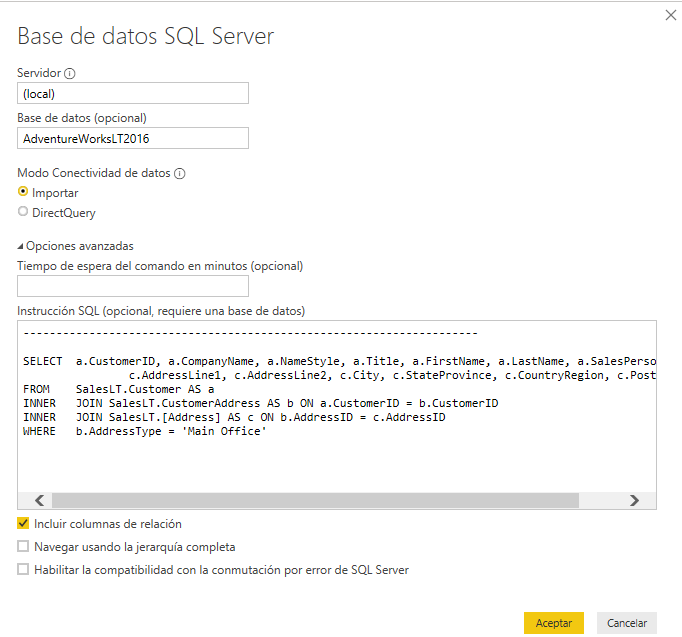
\includegraphics[width=15cm]{./Imagenes/img1} 
\end{center}


\item \textbf{Tarea 2: Graficar Datos}

\item \textbf{Tarea 3: Combinar Datos} 
\begin{center}
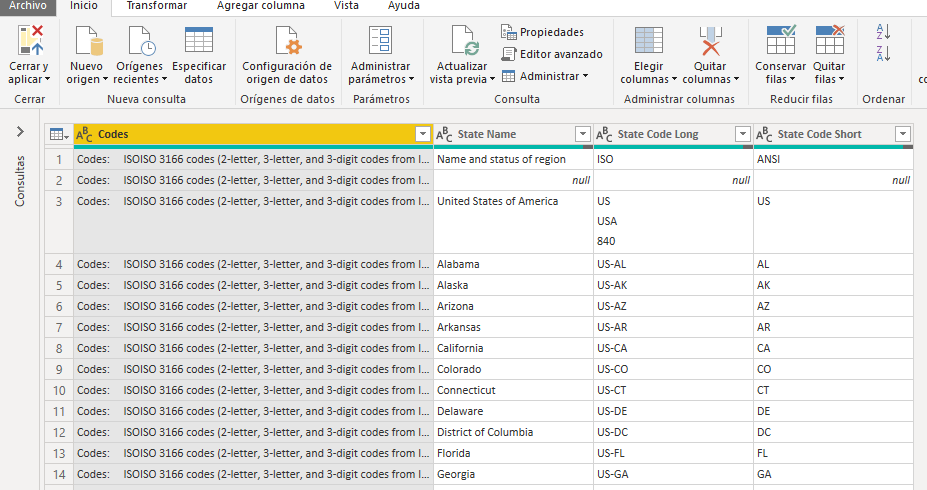
\includegraphics[width=15cm]{./Imagenes/2} 
\end{center}
\begin{center}
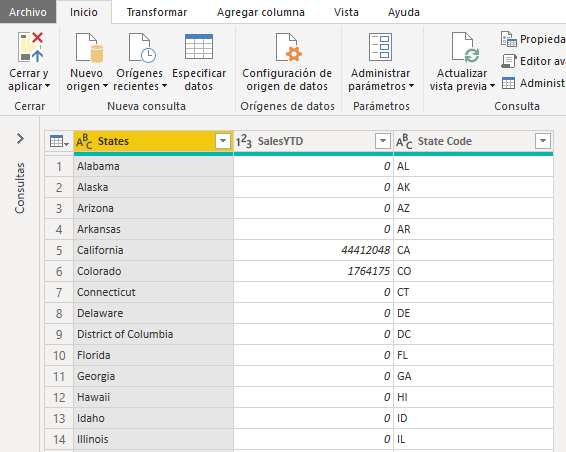
\includegraphics[width=15cm]{./Imagenes/3} 
\end{center}

\section*{Ejercicio 2: Construyendo Reportes en Power BI}
\item \textbf{Tarea 1: Crear un Gráfico}
\item \textbf{Tarea 2: Crear una Visualización de Mapa}
\textbf{}
\begin{center}
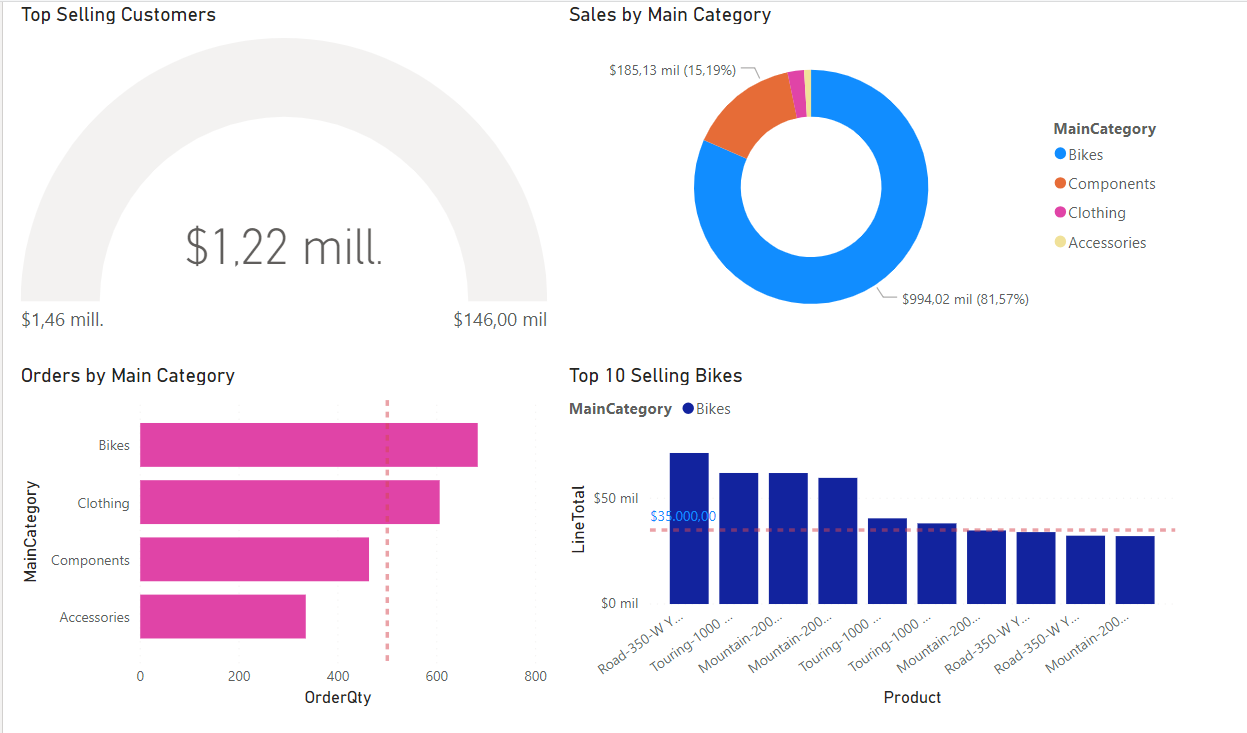
\includegraphics[width=15cm]{./Imagenes/img5} 
\end{center}
\textbf{}
\textbf{}
\begin{center}
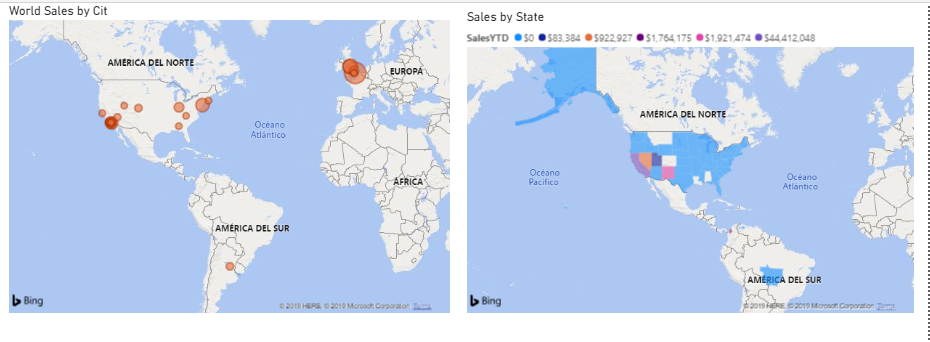
\includegraphics[width=15cm]{./Imagenes/5} 
\end{center}